\section{Istruzioni per l'uso}
\subsection{Requisiti di sistema}
Il server ospitante l'applicazione dovrà soddisfare alcuni requisiti di seguito elencati:
\begin{itemize}
\item Sistema operativo Linux o Mac OS;
\item 
\end{itemize}

\section{Files necessari}
Per procedere all'installazione dell'applicazione \emph{Premi} sono necessari alcuni file contenenti il codice sorgente.
Tali file sono reperibili all'interno del repository pubblico all'indirizzo \href{http://404notfoundunipd.github.io/premi/}{http://404notfoundunipd.github.io/premi/}, dove si troveranno tutte le istruzioni necessarie per scaricare i file dell'applicazione.

\section{Installazione}
\subsection{Linux}

\subsubsection{Installazione curl}
Curl è uno strumento per riga di comando e libreria per il trasferimento di dati con sintassi URL. \\
Per eseguire l'installazione è necessario scaricare il pacchetto d'installazione dal sito \href{http://curl.haxx.se/download.html}{http://curl.haxx.se/download.html}; una volta scaricato il pacchetto, estrarne i file in una cartella come nell'immagine seguente:

\begin{figure}[h]
\begin{center}
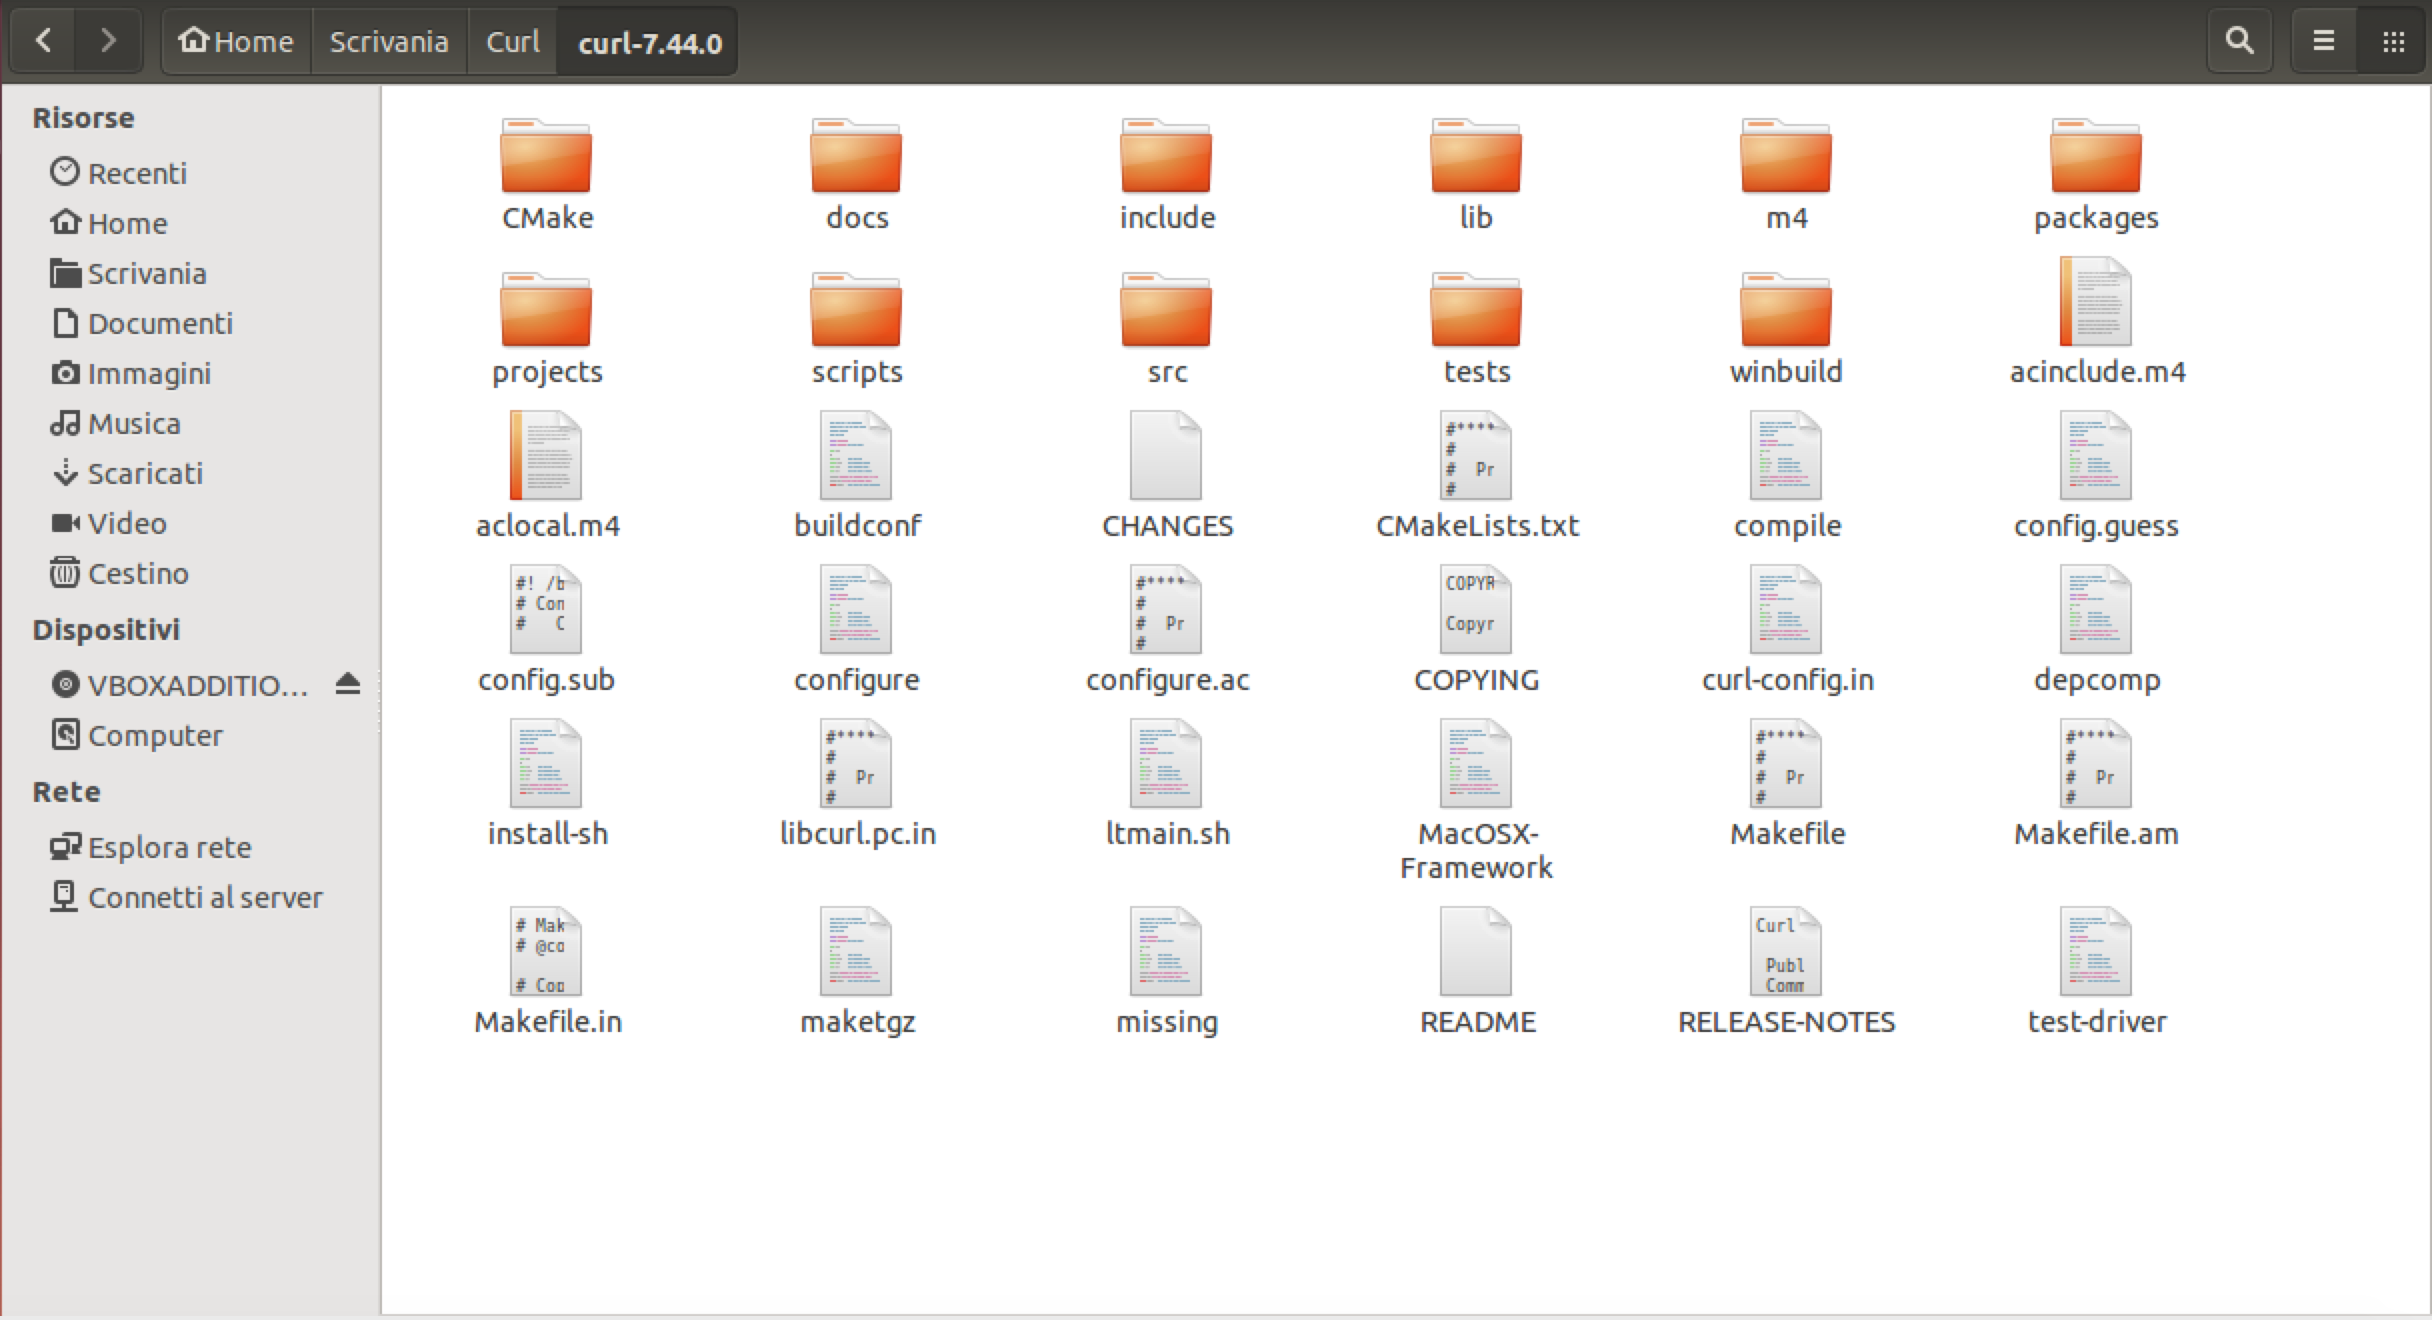
\includegraphics[scale=0.3]{img/curl_files_linux.png}
\caption{File \emph{curl} su ambiente linux.}
\end{center}
\end{figure}

\noindent Supponiamo ora di avere estratto i file all'interno della cartella \\
\verb+/home/notfound404/Desktop/Curl/curl-7.44.0/+.\\
Aprire quindi il terminale e spostarsi all'interno di questa cartella tramite il comando:

\begin{lstlisting}[style=DOS]
	$ cd /home/notfound404/Desktop/Curl/curl-7.44.0/
\end{lstlisting}

eseguire quindi in sequenza i comandi:

\begin{lstlisting}[style=DOS]
	$ ./configure
	$ make
	$ make test (optional)
	$ sudo make install
\end{lstlisting}
Se la procedura è andata a buon fine \emph{curl} sarà stato installato correttamente.

\subsubsection{Installazione MeteorJS}
\emph{MeteorJS} è una piattaforma completamente open source per lo sviluppo di applicazioni web o mobile in JavaScript.\\
Per eseguire la sua installazione sarà sufficiente aprire il terminale ed eseguire il comando:

\begin{lstlisting}[style=DOS]
	$ curl https://install.meteor.com/ | sh
\end{lstlisting}

Una volta terminata l'installazione, MeteorJs sarà pronto per essere utilizzato.

\subsubsection{Avvio applicazione}
Dopo aver scaricato l'archivio contenente i files necessari, come spiegato nella sezione \emph{3 Files necessari}, è necessario scompattarlo estraendone i files in una cartella, che per comodità supponiamo essere \verb+/home/notfound404/Desktop/Premi/+.\\
Per avviare l'applicazione aprire il terminale, spostarsi all'interno della cartella con il comando

\begin{lstlisting}[style=DOS]
	$ cd /home/notfound404/Desktop/Premi/
\end{lstlisting}

e avviare MeteorJs con il comando 

\begin{lstlisting}[style=DOS]
	$ sudo meteor
\end{lstlisting}

\begin{figure}[!h]
\begin{center}
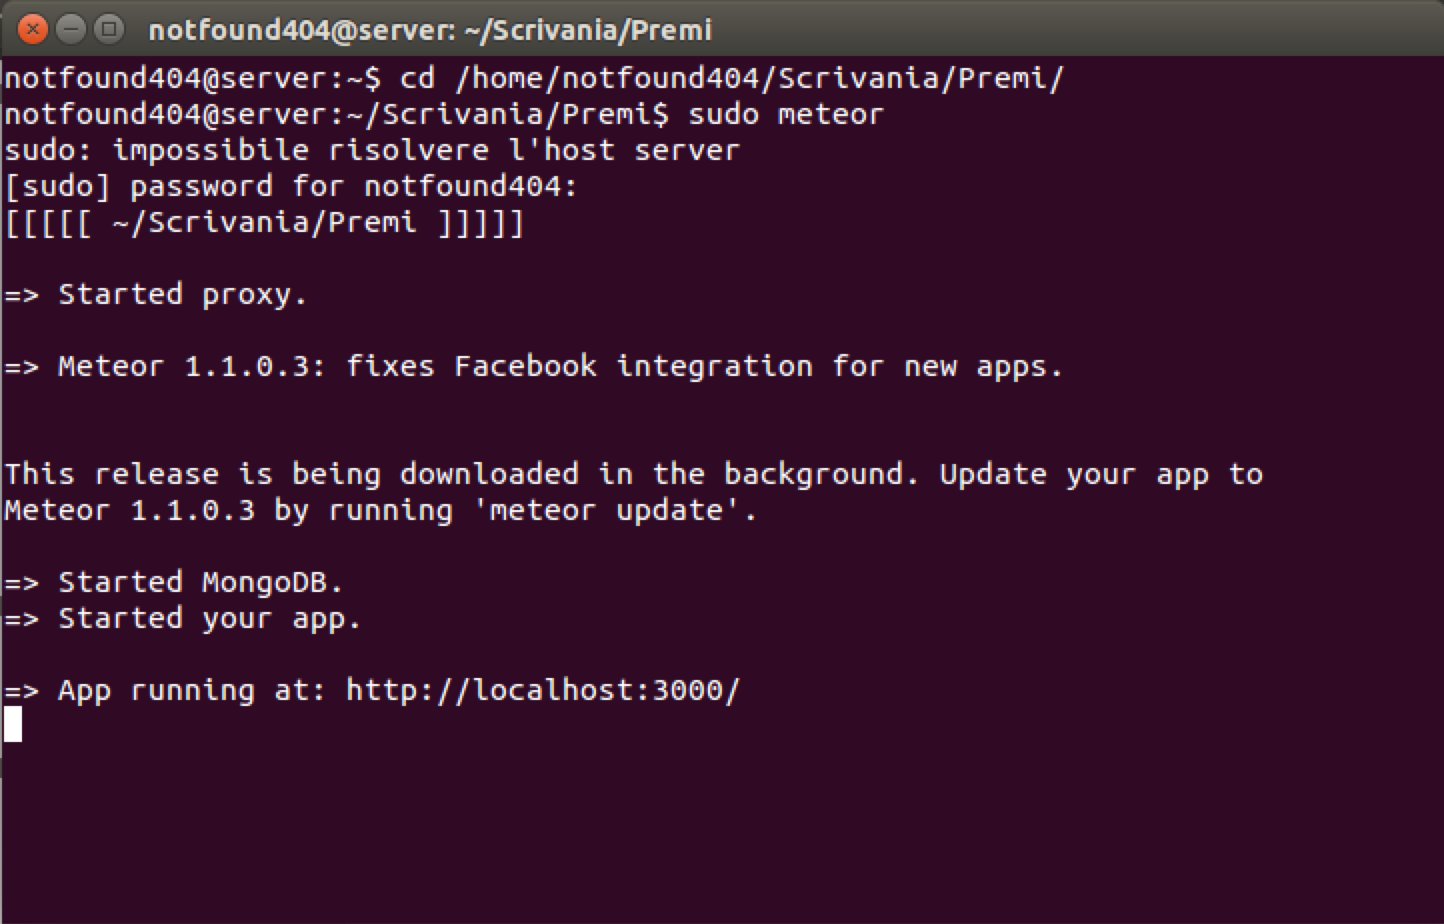
\includegraphics[scale=0.4]{img/start_premi.png}
\caption{Avvio applicazione.}
\end{center}
\end{figure}

\newpage
Nel caso vengano riscontrati errori verificare i seguenti punti:
\begin{itemize}
\item connettività ad internet; potrebbe essere necessario il download di alcuni pacchetti mancanti in seguito al primo avvio dell'applicazione;
\item controllare che all'interno della cartella \emph{Premi}, contenente i files dell'applicazione, sia presente anche la cartella \verb+.meteor+, sarà necessario abilitare la visualizzazione dei files nascosti;
\item verificare di disporre i privilegi di amministratore.
\end{itemize}

\noindent Nel caso in cui nessuna delle soluzioni sopra indicate porti ad una soluzione del problema, contattare gli sviluppatori attraverso le modalità indicate nella sezione \emph{1.5 Assistenza tecnica} del documento corrente.\\

Se invece l'applicazione è stata avviata correttamente verrà visualizzato sul terminale il messaggio 

\begin{lstlisting}[style=DOS]
	$ => App running at: http://localhost:3000/
\end{lstlisting}

Sarà quindi sufficiente aprire il browser Google Chrome ed inserire nella barra degli indirizzi \verb+http://localhost:3000/+ oppure \verb+http://127.0.0.1:3000/+.


\subsection{Mac OS}
\subsubsection{Installazione curl}

\subsubsection{Installazione MeteorJS}

\subsubsection{Avvio applicazione}

\section{Consigli}